\section{Sistema perturbado y filtros}
Con el fin de tener un modelo que emule de una mejor manera el mundo real,
se decidío introducir perturbar el sistema, tanto en la entrada (con el fin
de reproducir el error de medida y eventualidades que pueden afectar el
sistema) como en la salida (nuevamente para simular los erroes de medida).
Para perturbar la señal de entrada se optó por utilizar un ruido blanco
con periodo de muestreo $0.1$ y potencia $0.01$. La entrada perturbada se puede
ver en la figura~\ref{fig:entrada-ruido}

\begin{figure}[t]
  \label{fig:entrada-ruido}
  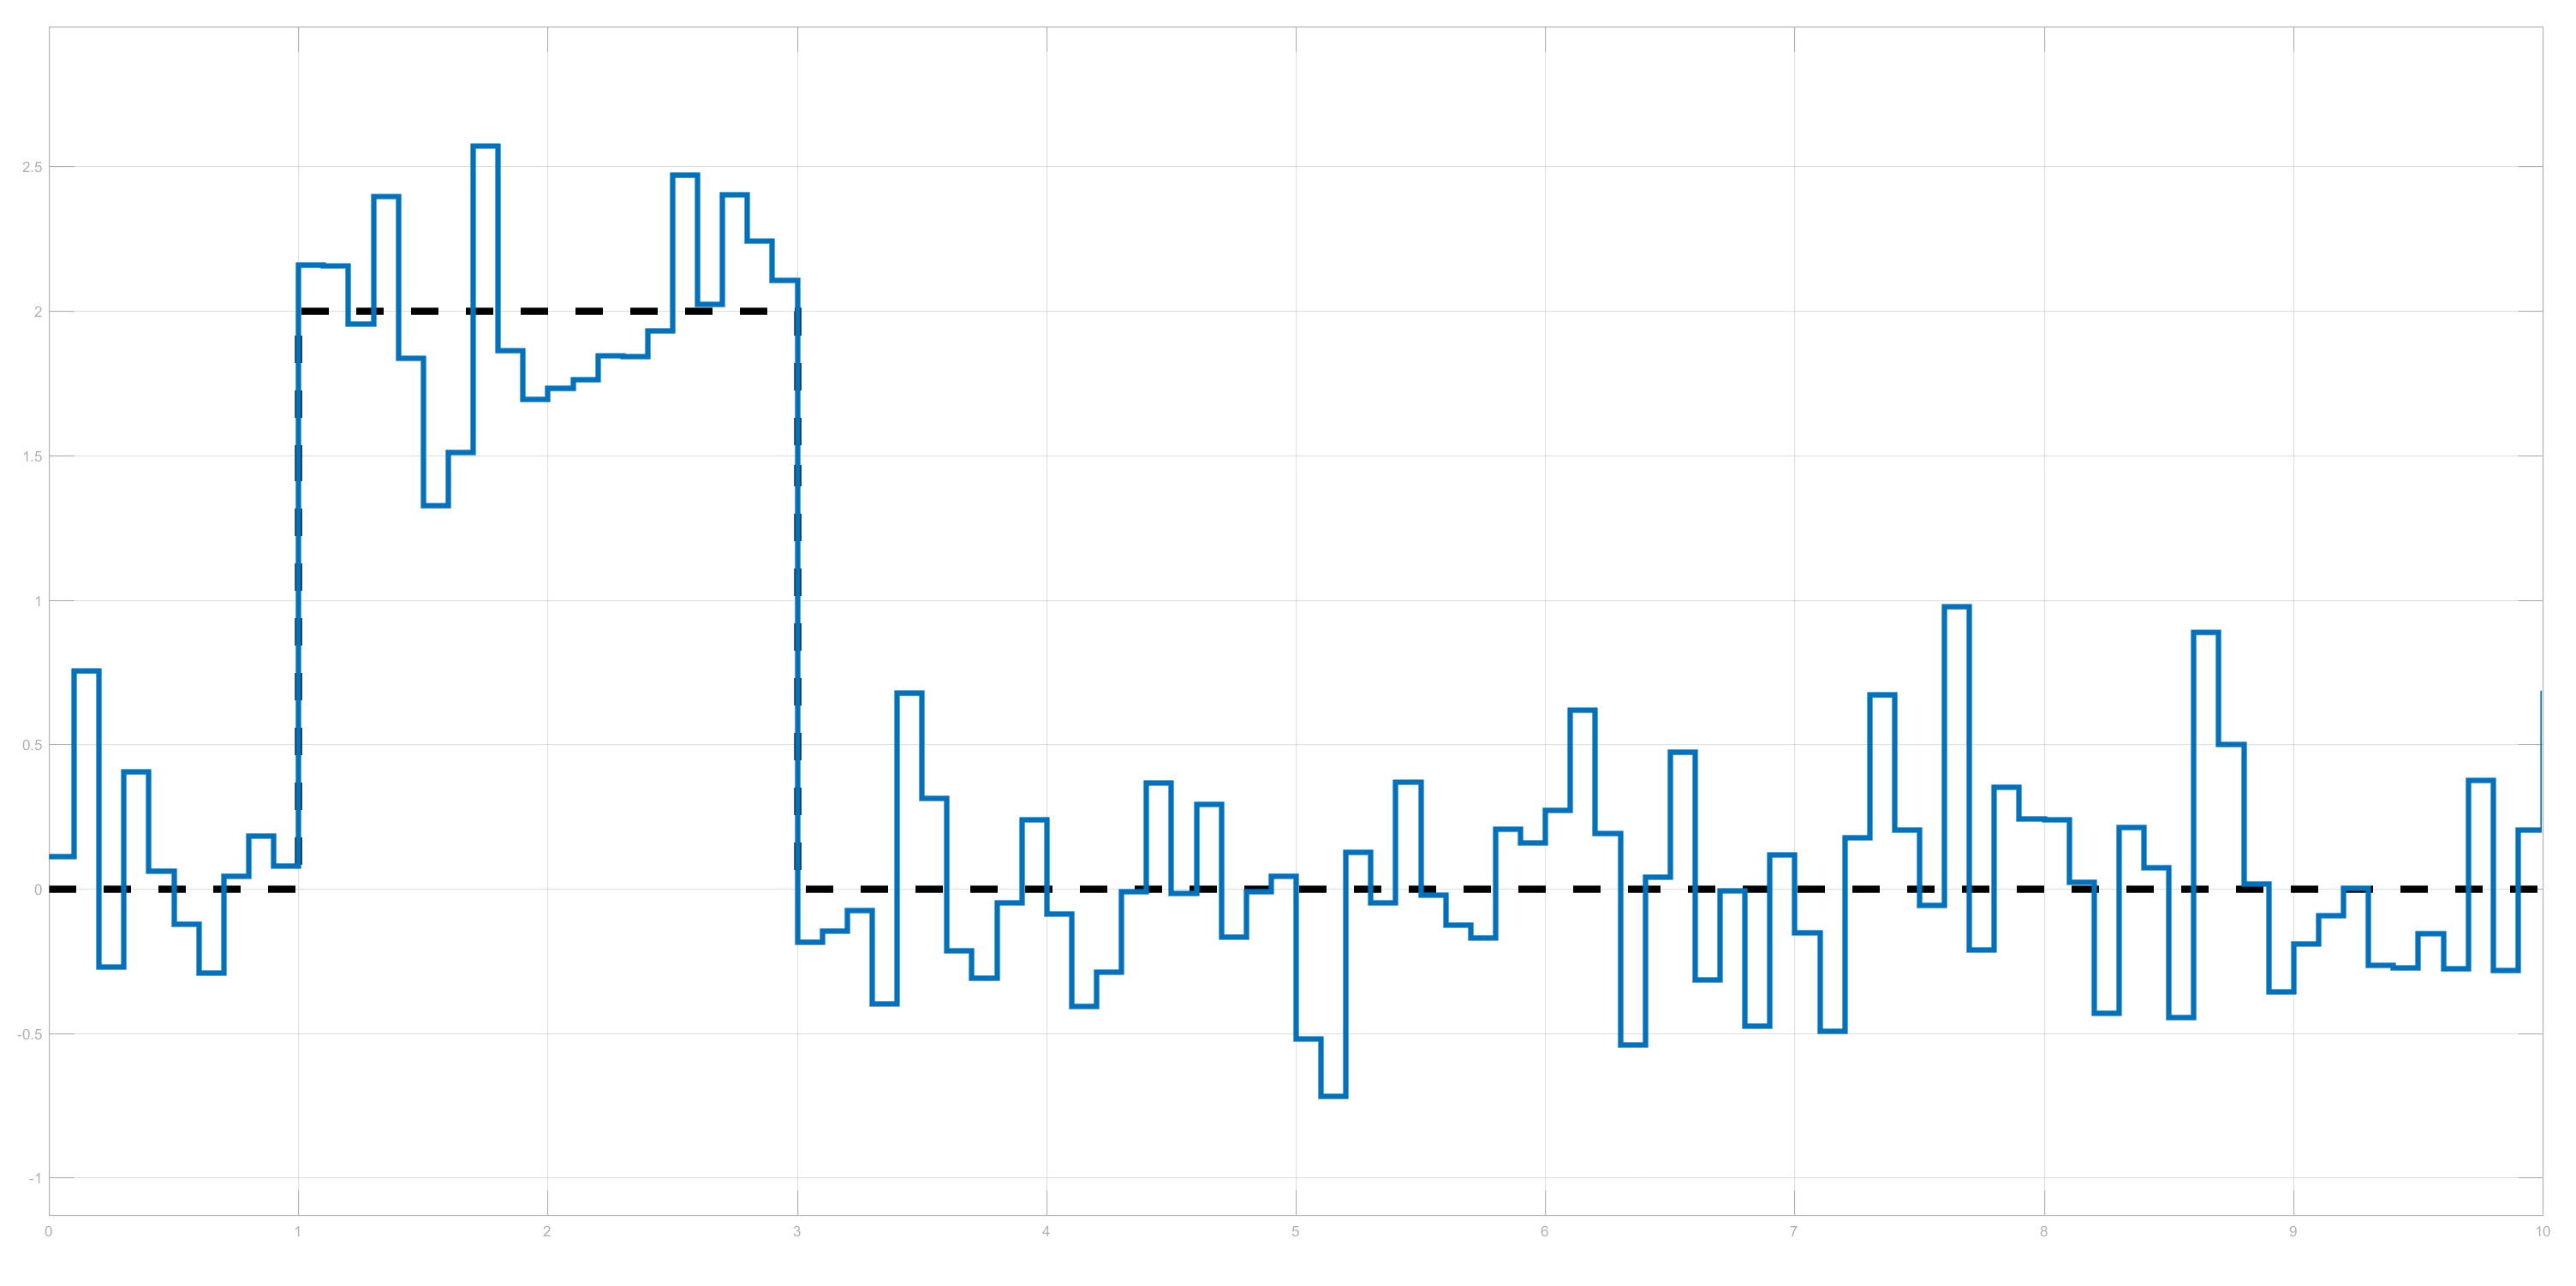
\includegraphics[scale=1]{Figuras/entrada}
  \caption{Señal de entrada perturbada.} 
\end{figure}

Esta señal entra al sistema y la salida que esté genera tambien se ver
perturbado, esta vez, por una suma de señales senoidales de alta frecuencia.
Posteriormente esta señal se ve sometida a un filtro pasabajas de primer orden
(el debería eliminar el ruido)

La literatura señala que la funcion de transferencia de dicho tipo de filtros
son de la forma~\citep{filtros}:
\[
\frac{1}{\tau s + 1}
\]

Donde $\tau $ es un parametro que depende de la frecuencia que se desea filtrar,
en particular para nuestro problema se decidió escoger $\frac{1}{15}$.

